%%%%%%%%%%%%%%%%%%%%%%%%%%%%%%%%%%%%%%%%%%%%%%%%%%%%%%%%%
%%%%%%%%%%%%%%%%%%%%%%%%%%%%----->SECCIÓN 3<-----%%%%%%%%%%%%%%%%%%%%%%%%%
\newpage
\newpage

\chapter{El Observatorio Pierre Auger}

El Observatorio Pierre Auger es el observatorio de CR más grande del mundo, con un área de detección de alrededor de $3000 km^{2}$. Su objetivo principal es detectar CR de ultra alta energía $(E > 10^{18} eV)$, cuya tasa de arribo a la tierra está entre 1 partícula $km^{2}/year$ a 1 partícula $km^{2}/century$. El observatorio es un arreglo híbrido, que está constituido principalmente por dos tipos de detectores: los telescopios de fluorescencia atmosférica y los detectores Cherenkov de superficie. Este detector híbrido proporciona estadísticas de alto nivel y reduce las incertidumbres sistemáticas en la medición de las energías de los CR \cite{allekotte_2008}. En este capítulo, revisaremos las generalidades de cada uno de estos detectores, enfocándonos en los detectores de superficie y sus mecanismos para la identificación de partículas.

\section{Detector de Fluorescencia}
El detector de fluorescencia está diseñado para registrar el desarrollo longitudinal de las lluvias de partículas secundarias generadas por CR de muy alta energía. Esto es posible gracias a que al propagarse por la atmósfera los CR secundarios excitan el nitrógeno liberando luz fluorescente en el rango de 300 nm a 430 nm. El criterio principal de su diseño es la detección de cada lluvia con energías de al menos $10^{19}eV$ (\cite{FD_auger}). Este arreglo consta de 24 telescopios independientes distribuidos en 4 sitios, cada uno con un campo de visión de $30^{\circ} \times 30^{\circ}$  como se observa en la figura \ref{fd_auger}. En este instrumento, el número de fotones producidos es proporcional a la energía de la componente electromagnética de la lluvia y al número total de partículas generadas a cierta profundidad atmosférica (\cite{FD_auger}).

\begin{figure}[!ht]
\centering
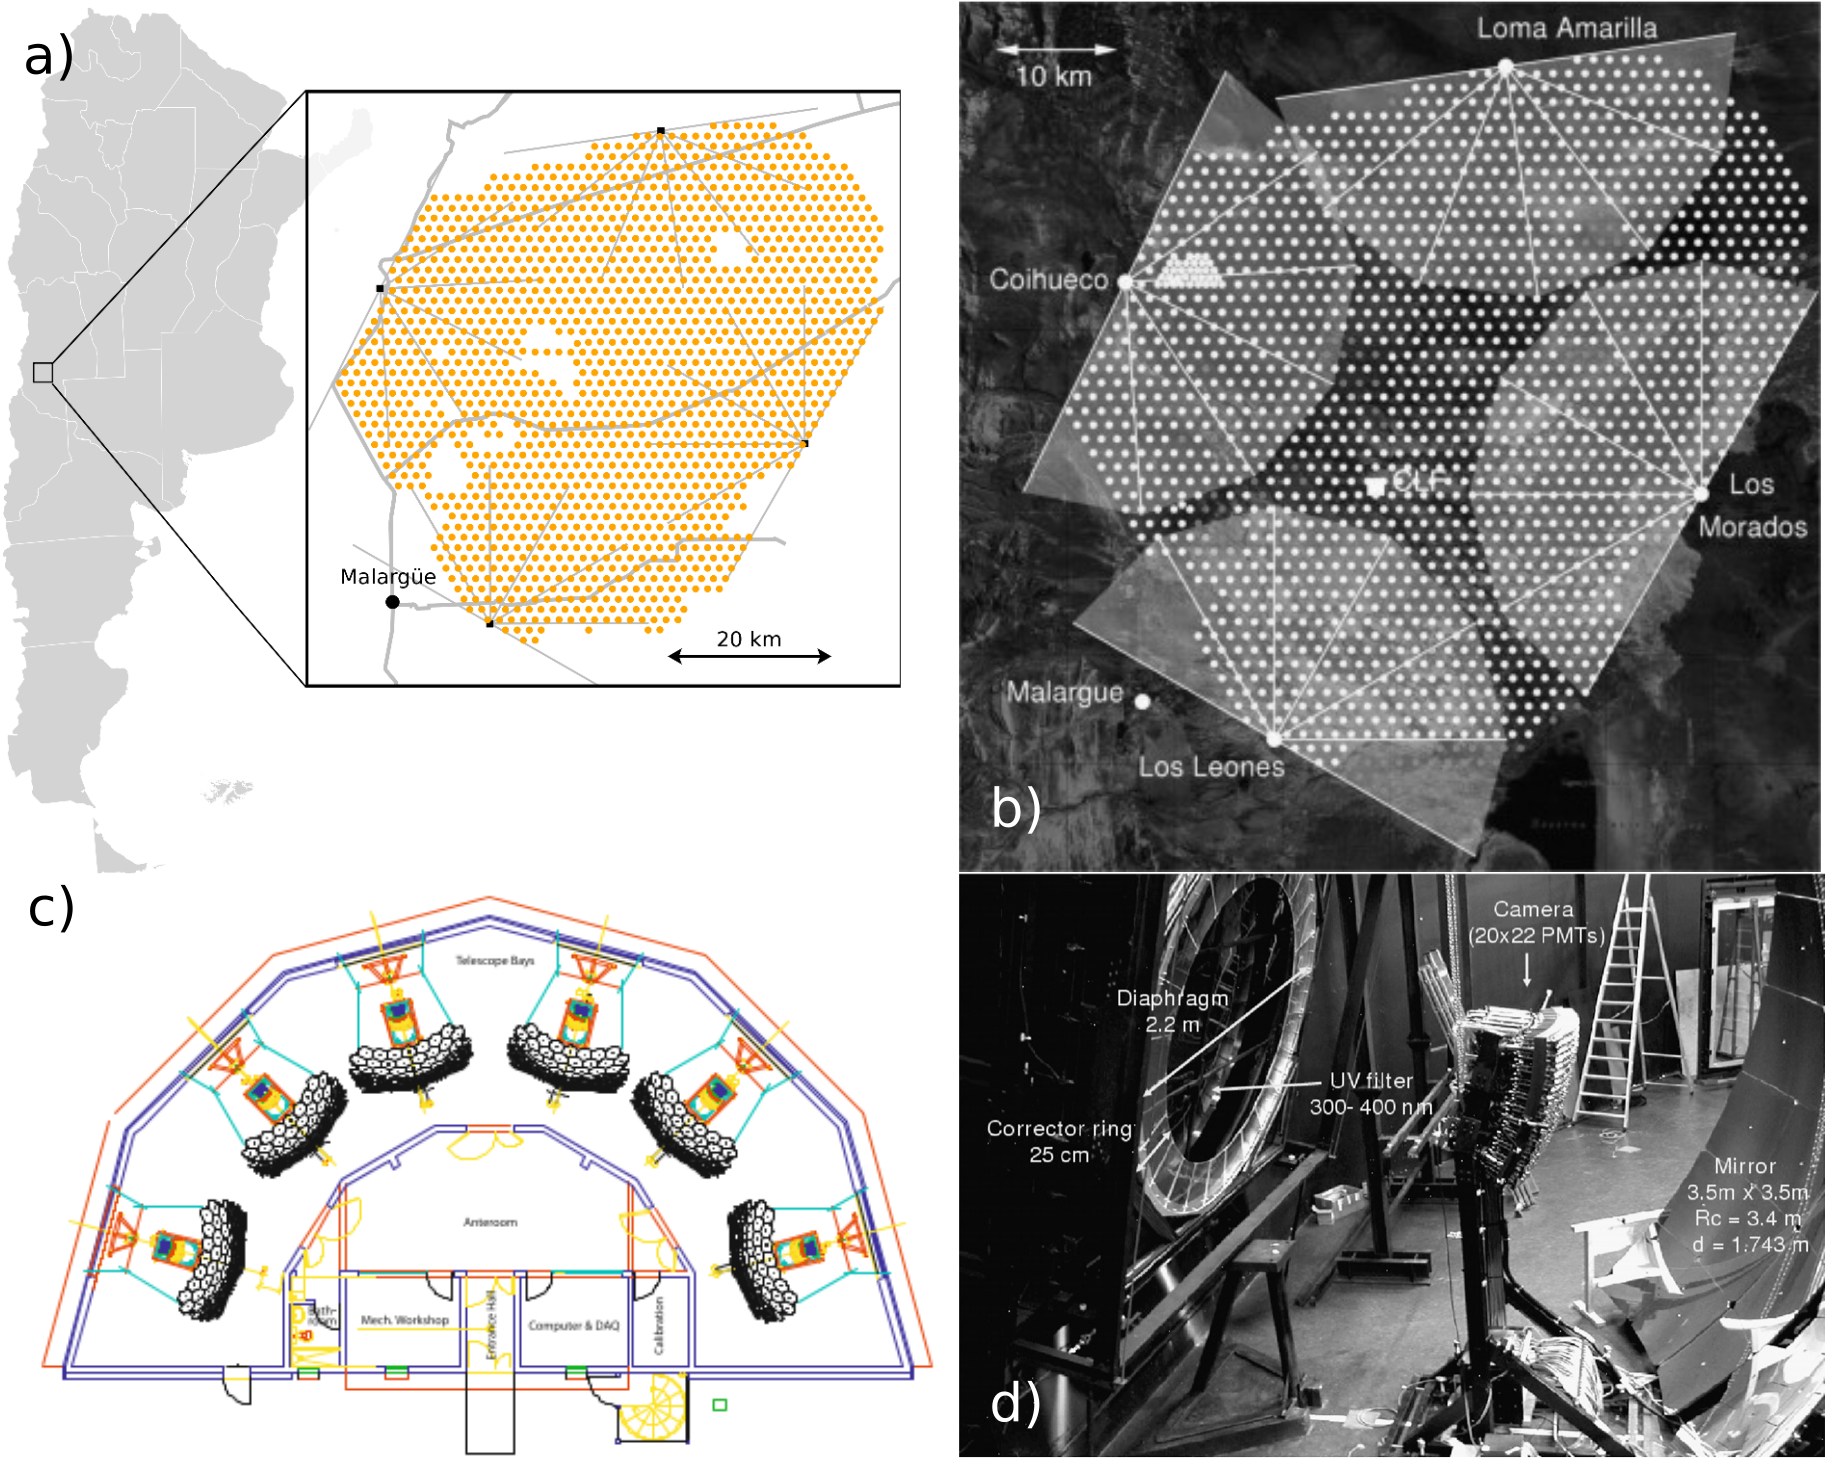
\includegraphics[width=1\textwidth]{Figs/FD_auger_composition.png}
\caption{a) Mapa donde se muestra la ubicación del Observatorio Pierre Auger y sus sistemas detectores. Los puntos amarillos corresponden a los detectores de superficie, y los 4 puntos negros en las fronteras, corresponden a la ubicación de los detectores de fluorescencia (\cite{asorey_2012}). b) Los puntos grises muestran las posiciones de las estaciones de detectores de superficie. Los semicírculos en gris claro indican los campos de visión de 24 telescopios de fluorescencia situados en cuatro edificios en el perímetro de los detectores de superficie (\cite{FD_auger}). c) Esquema de uno de los cuatro edificios con seis telescopios de fluorescencia en su interior logrando un campo de visión de $180^{o}$ (\cite{FD_auger}). d) Estructura de un telescopio de fluorescencia. El sistema de apertura consta de un diafragma, un anillo corrector y un filtro UV. Los componentes ópticos que corresponden al espejo, la cámara y un conjunto de 20x22 PMT (\cite{dedonato_2007}).}
\label{fd_auger}
\end{figure}

El arreglo utiliza un filtro UV para dejar pasar solo luz ultravioleta en el rango de 330 nm a 380 nm que corresponde al rango de interés para las observaciones. Además, los telescopios están diseñados para funcionar únicamente durante noches despejadas sin Luna, lo que reduce el ruido de fondo y mejora la precisión de las mediciones. 

\section{Detector de superficie}

El Observatorio cuenta con un detector de superficie que comprende una matriz de 1660 estaciones de detectores Cherenkov de agua (WCD) abarcando un área total de $3000$ $km^{2}$. Estas estaciones están distribuidas en una red hexagonal de $1.5$ $km$ de espaciado (ver figura \ref{fd_auger}). Dicha configuración está diseñada para estudiar el desarrollo transversal de todas las lluvias de partículas generadas por primarios de al menos $10^{18}$ $eV$ a nivel del suelo.

Dado el tamaño del área cubierta, las estaciones deben operar de manera autónoma y requerir poco mantenimiento (\cite{allekotte_2008}). Por lo tanto, estos detectores están interconectados a través de una red inalámbrica de área local, cuyo receptor principal es el telescopio de fluorescencia más cercano, que se encarga de transmitir los datos a la central de recopilación principal CDAS.

\subsection{Efecto Cherenkov}

Cuando una partícula con carga se mueve a través de un medio, su pérdida de energía aumentará a medida que la densidad del medio se incremente. Si consideramos que la densidad $\rho$ del medio es constante y que \textit{b} es el parámetro de impacto, la energía que pierde la partícula al atravesar una sección de longitud \textit{dl} dentro de un cilindro de radio \textit{a}, cuyo eje coincide con la dirección de movimiento, se puede expresar como $\frac{dE}{dl} = \rho \frac{dE}{dX}$. Esta pérdida de energía está determinada por el flujo del vector de Poynting, con la componente longitudinal $E_{1}$ del campo eléctrico, y con la componente transversal del campo magnético $B_{3}$ presentes en el medio, en función de la frecuencia $\omega$ (\cite{fermi_1940}).
\begin{equation}
    \frac{dE}{dl} = -ca \mathcal{R}\left(\int_{0}^{\infty} B^{*}E_{1}(\omega) \, d\omega\right)
    \label{fermi1}
\end{equation}
%%%%%%%%%%%%%%%%% PARENTESISSSSS
Consideremos una partícula cargada que se desplaza a una velocidad $v=\beta c$ a través de un medio con una constante dieléctrica $\epsilon(\omega)$ y un número atómico $Z$. En este escenario, la longitud de onda de la radiación emitida se modificará debido a la presencia del medio de la siguiente manera:
\begin{equation}
\lambda^{2}=\frac{\omega^{2}}{v^{2}}(1-\beta^{2}\epsilon(\omega)).
\label{lamdamod}
\end{equation}
Teniendo en cuenta las expresiones para los campos $E$ y $B$, el integrando de la ecuación \ref{fermi1} obtenemos:
\begin{equation}
B^{*}_{3}(\omega)E_{1}(\omega)=\left(\frac{Ze}{c}\right)^2 \left(-i\sqrt{\frac{\lambda^{*}}{\lambda}}\right)\left(1-\frac{1}{\beta^{2}\epsilon(\omega)}\right)exp[-a(\lambda+\lambda^{*})]\omega.
\end{equation}
En este caso, si $\lambda$ es un número imaginario puro, $\lambda^{*}=-\lambda$ lo que haría 
$exp[-a(\lambda+\lambda^{*})] = 1$ y por consiguiente la expresión \ref{fermi1} sería independiente de $a$, donde parte de la energía escapa al infinito en forma de emisión coherente de radiación (\cite{asorey_2012}). Esto sucede si $\epsilon$ es real, es decir que el medio no es absorbente y que $\beta^{2}\epsilon(\omega)>1$ ó $\beta=\frac{1}{\sqrt{\epsilon(\omega)}}$. En otras palabras, si la velocidad de la partícula cargada es mayor que la velocidad de la luz en el medio a una frecuencia $\omega$, fenómeno conocido como \textit{Efecto Cherenkov} (\cite{asorey_2012}).

Si el medio es ligeramente absorbente la expresión \ref{fermi1} queda como:
\begin{equation}
\left(\frac{dE}{dl}\right)_{Cherenkov}=\left(\frac{Ze}{c}\right)^{2}\int_{\beta^{2}\epsilon(\omega)>1} \omega\left(1-\frac{1}{\beta^{2}\epsilon(\omega)}\right)d\omega
\end{equation}
donde se observa que la emisión de radiación depende de la frecuencia. En el caso del agua, en el espectro visible, la radiación Cherenkov se produce a longitudes de onda cortas, donde  $n(\omega) \approx \sqrt{\epsilon(\omega)}$ aumenta levemente con la frecuencia. El ángulo de emisión de la radiación está definido entonces por:
\begin{equation}
cos\theta_{c}=\frac{1}{\beta\sqrt{\epsilon(\omega)}},
\end{equation}
Para el rango de frecuencias de interés (cerca del ultravioleta), el valor del índice de refracción puede ser considerado constante, con lo que podemos obtener el número de fotones Cherenkov producidos en un intervalo de longitudes de onda como sigue,
\begin{equation}
N=2\pi \alpha_{EM}l\left(1-\frac{1}{\beta^{2}n^{2}}\right)\left(\frac{1}{\lambda_{2}}-\frac{1}{\lambda_{1}}\right).
\label{cherenkovnumber}
\end{equation}


%%%%%%%%%%%%%%%%% PARENTESISSSSS

%EN ALGÚN MOMENTO DE LA VIDA \hbar cambió por \hslash en esta joda y no me enteré....

Donde $\alpha_{EM}=(e^2/ \hslash c)$ es la constante de estructura fina. Además, el momento de una partícula con masa en reposo $m_{0}$ y velocidad $\beta c$ es $p\equiv mv = \beta \gamma m_{0}c$, lo que permite calcular el número de fotones emitidos por una partícula con momento $p$ al recorrer una longitud $l$ en un medio con índice de refracción $n$. En el caso de los tubos fotomultiplicadores (PMT) utilizados en el Observatorio Pierre Auger, que son sensibles al rango de $300 - 570nm$, es posible definir dos propiedades clave en la respuesta posterior de los detectores Cherenkov:
\begin{itemize}
\item La radiación solo se emite cuando $\beta>1/n$.
\item El número de fotones emitidos por unidad de longitud tiende a un valor constante (ver figura \ref{stopping_cherenkov}), que solo depende del rango de longitudes de onda considerado, del índice de refracción del medio y la distancia recorrida en dicho medio. De esta manera, la señal en el detector no proviene de la energía depositada, sino de la cantidad de fotones producidos, es decir, de la distancia recorrida por la partícula en el agua (\cite{asorey_2012}).
\end{itemize}
\begin{figure}
\centering
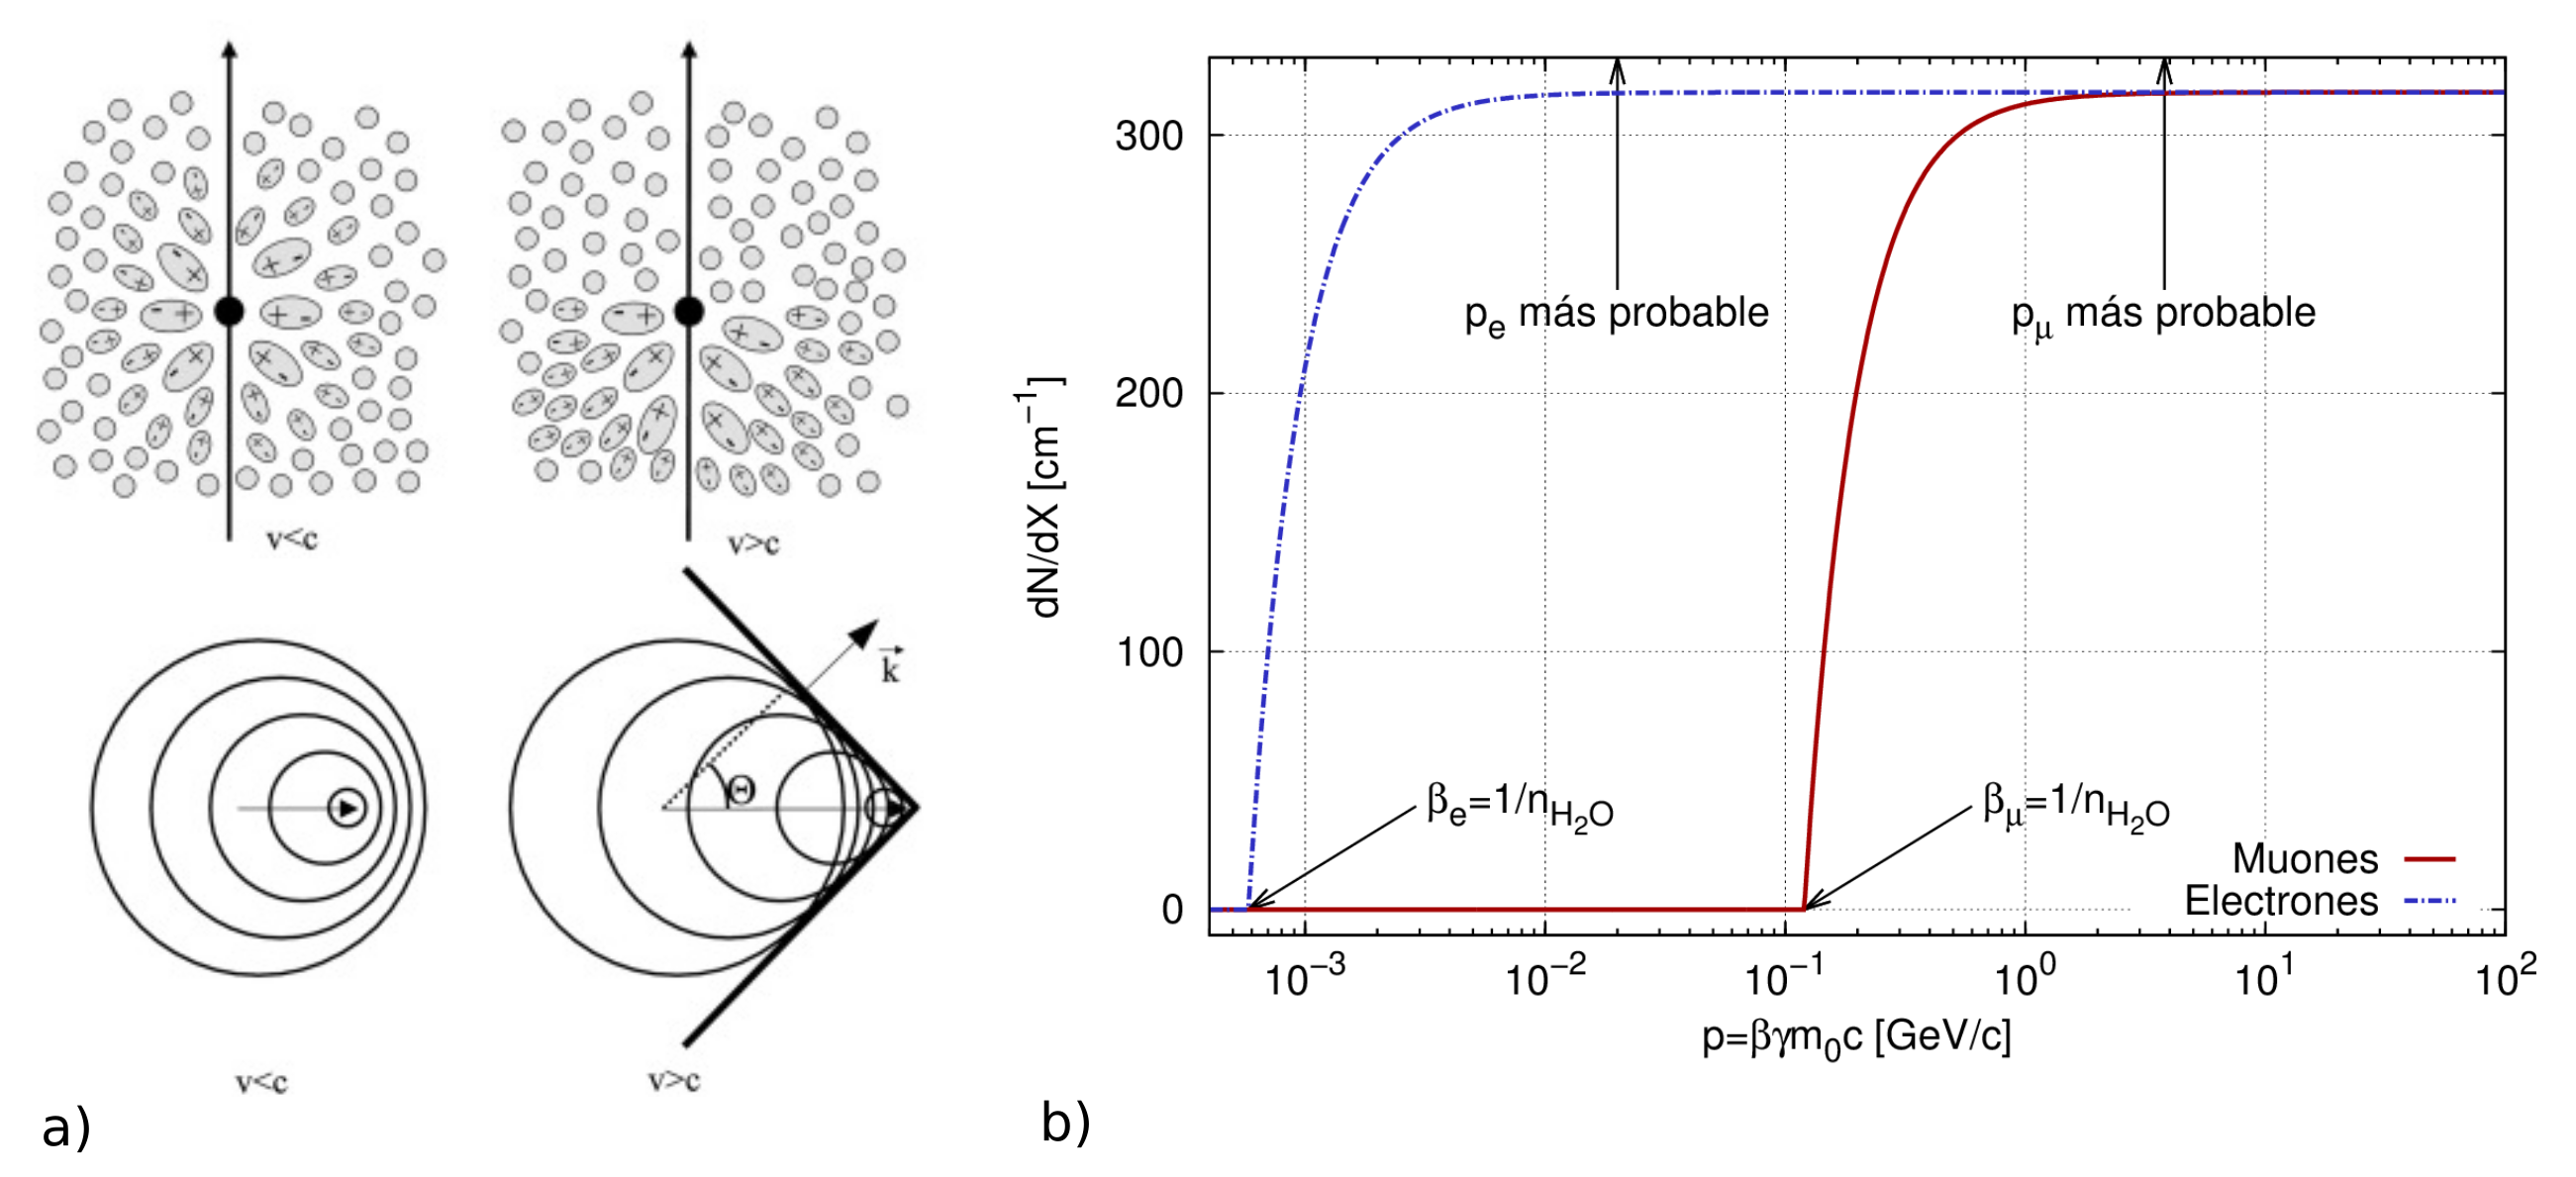
\includegraphics[width=1\textwidth]{Figs/cherenkov_stopping.png}
\caption{a) Arriba: ilustración de la polarización del medio inducida por el paso de una partícula relativista. Abajo: Construcción del frente de onda de Cherenkov. Fuente: \cite{deNaurois:2015oda} b) Esquema Producción de fotones Cherenkov en la banda $300 nm < \lambda < 570 nm$ según la ecuación \ref{cherenkovnumber} como función del impulso. La línea punteada corresponde a un electrón y la sólida a un muón luego de haber recorrido 1 cm en agua líquida. Se puede observar que la cantidad de fotones tiende rápidamente a un valor constante de $\thicksim 315$ fotones por centímetro incluyendo el momento más probable para las dos partículas. Fuente \cite{asorey_2012}}
\label{stopping_cherenkov}
\end{figure}
\subsection{El detector Cherenkov}
 
%Para ampliar las capacidades del observatorio a energías más bajas, también se despliega una región de relleno de estaciones SD con un espaciado de 750 m (SD-750) [68]. 
Cada detector de superficie se compone de un recipiente cilíndrico con una base de 10 $m^{2}$, lleno con 12 $m^{3}$ de agua de alta pureza que permite una mínima absorción de luz ultravioleta cercana. Esta agua se encuentra dentro de una bolsa fabricada con Tyvek, un material reflectante (ver figura \ref{fig:SD_auger}). Cuando las partículas relativistas atraviesan el volumen de agua, generan radiación Cherenkov que es reflejada y dispersada por el Tyvek en el interior del recipiente, lo que incrementa la probabilidad de detección (\cite{allekotte_2008}).

Esta radiación es captada por tres PMT Photonis XP1805/D1 de 9 pulgadas de diámetro (\cite{bertou_2006},\cite{allekotte_2008}), dispuestos de forma simétrica en la parte superior del tanque. Las señales analógicas de los PMT son convertidas a formato digital en la electrónica de la estación mediante convertidores de tipo flash de analógico a digital (FADC). Cada PMT registra el pulso que genera la detección de fotoelectrones que se caracteriza por tener un crecimiento rápido y un posterior decaimiento exponencial como se muestra en la figura \ref{fig:PMT} (\cite{asorey_2012}).

%Cada SD consta de un tanque cilíndrico de 10$m^{2}$ de base con 12 $m^{3}$ de agua ultra pura que permita una baja absorción del ultravioleta cercano, dentro de una bolsa con un material reflectante realizada en Tyvek. La radiación Cherenkov producida por el paso de partículas relativistas a través del volumen de agua, es reflejada y difundida por el Tyvek en el interior, maximizando la probabilidad de detección \cite{asorey_2012} y es registrada con tresPMT(PMT) Photonis XP1805/D1 de 9 pulgadas de diámetro, (\cite{Aab_2015}) colocados simétricamente en la parte superior del tanque. Las señales analógicas provenientes de los PMT son digitalizadas en la electrónica de las estación mediante conversores analógicos digitales tipo flash (FADC).
\begin{figure}[!ht]
  \centering
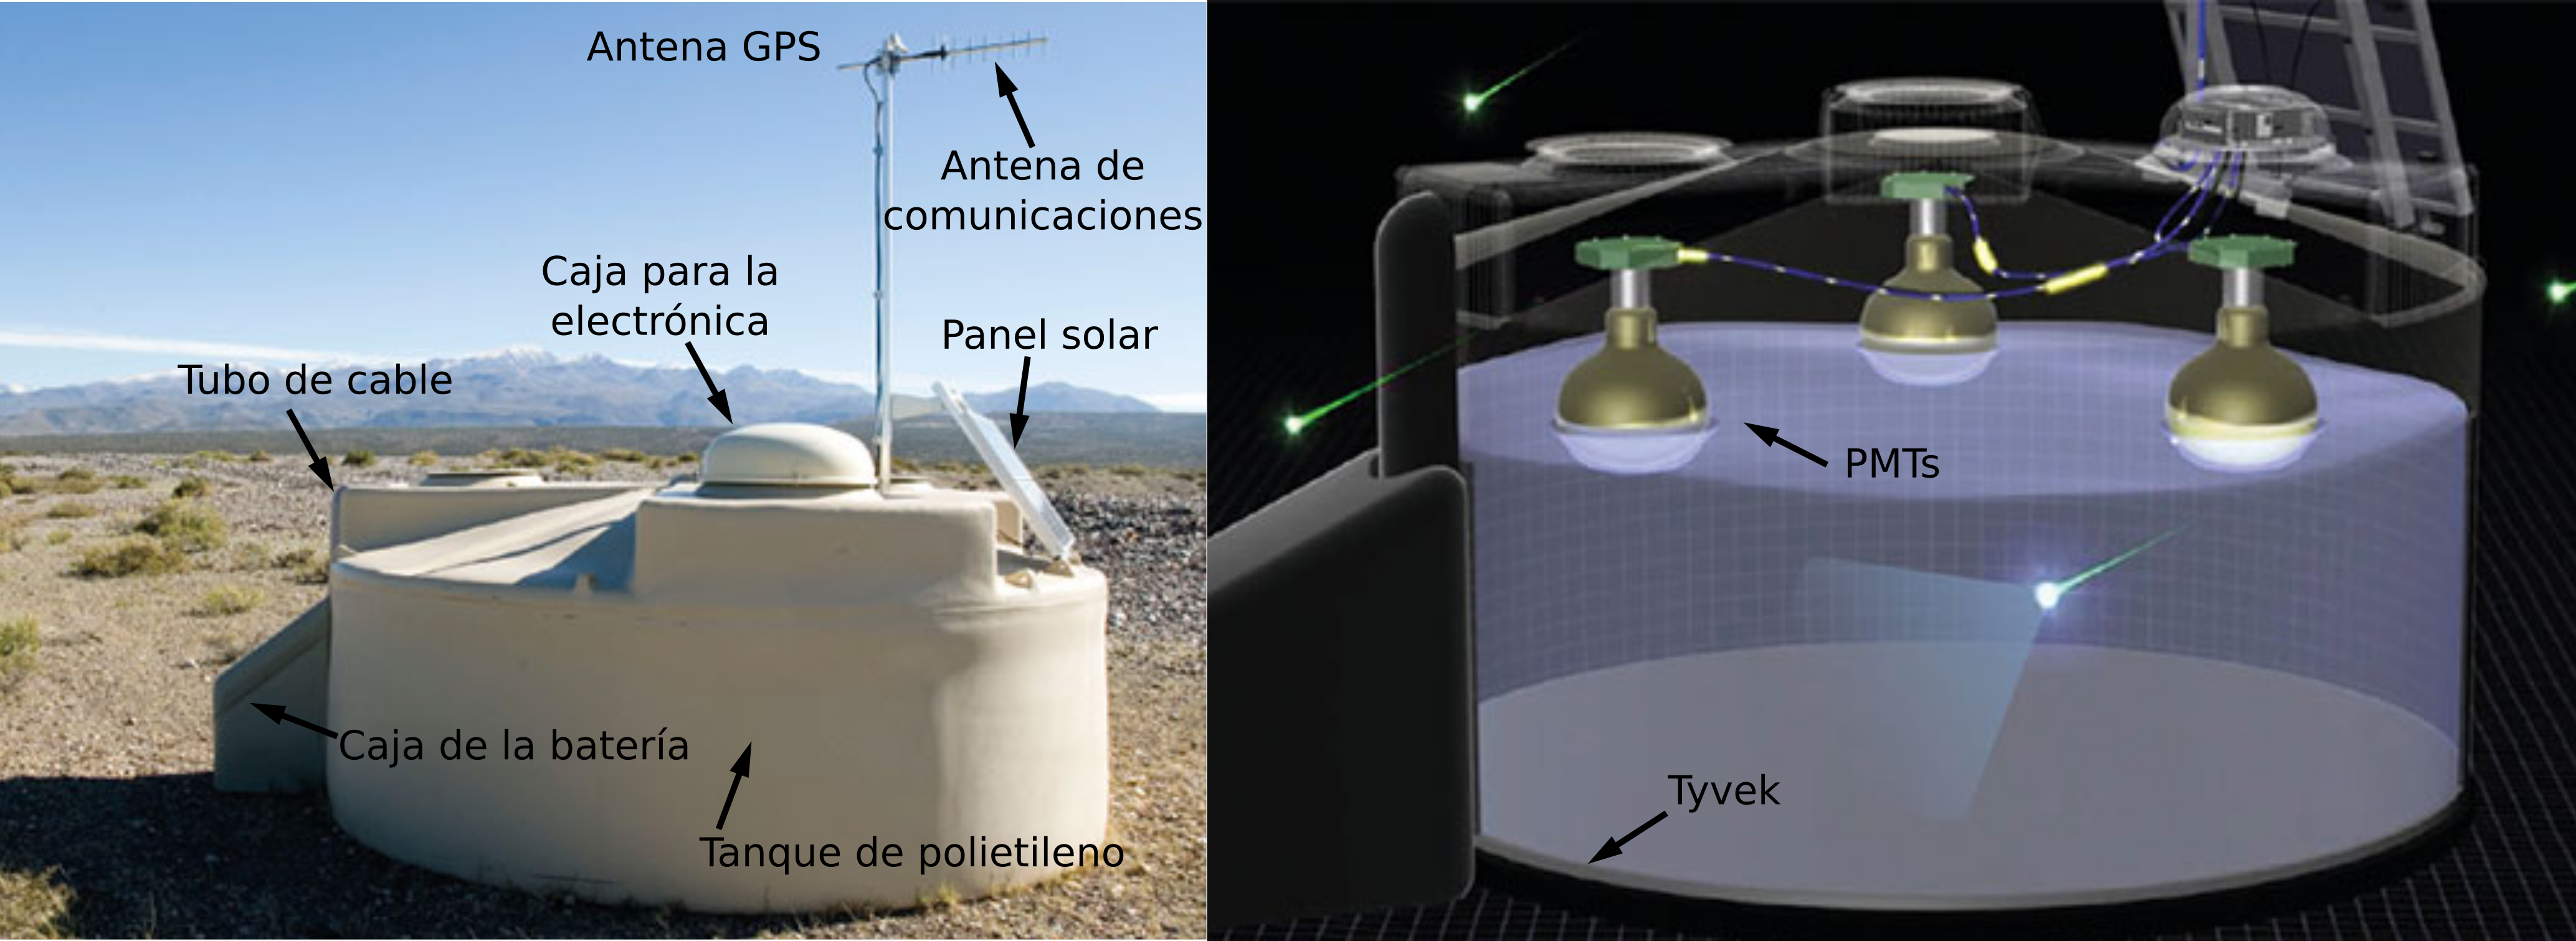
\includegraphics[width=0.8\textwidth]{Figs/SD_componentes.png}
  \caption{Estructura de un detector de superficie. A la izquierda se observa el exterior de un detector WCD del Observatorio ubicado en la Pampa Amarilla. A la derecha vemos una representación de su interior: Al entrar la partícula cargada al agua se produce un cono de luz Cherenkov, estos fotones son reflejados por las paredes del detector y recogidos por los PMT ubicados simétricamente en la superficie superior. \cite{allekotte_2008}}
  \label{fig:SD_auger}
\end{figure}



\begin{figure}[h!]
  \centering
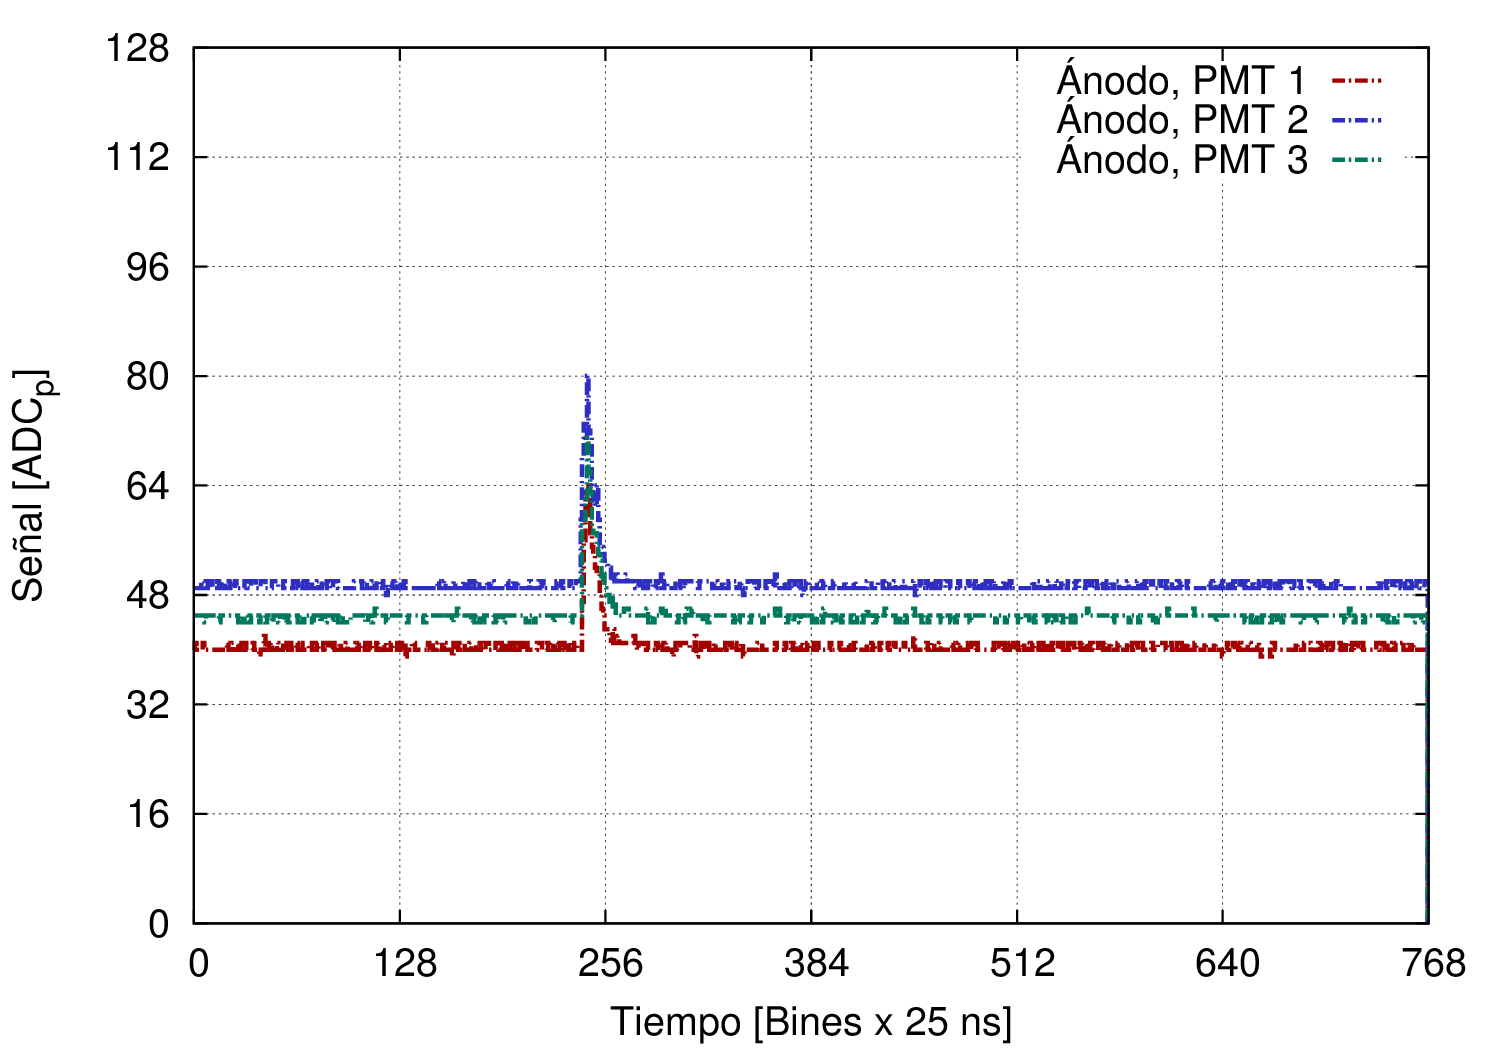
\includegraphics[width=0.6\textwidth]{Figs/PMTs_signal.png}
  \caption{Señal del ánodo de cada PMT. Estas señales son digitalizadas mediante seis conversores FADC de 10 bits a una velocidad de muestreo de 40 MHz. La traza consiste en un bloque contiguo de 768 bines de señal de 25 ns cada uno, totalizando $19.2 \mu s$. Fuente: (\cite{asorey_2012})}
  \label{fig:PMT}
\end{figure}
Una de las ventajas de usar detectores Cherenkov es que se puede diferenciar el paso de los muones (o su decaimiento) y la absorción de los electrones. Los muones atmosféricos (con energías típicas de $E_\mu \thicksim 3GeV$), depositan en el detector solo una pequeña fracción de su energía cinética de tal forma que son capaces de atravesarlo (\cite{asorey_2012}). La señal Cherenkov producida por muones depende únicamente de la longitud recorrida en el agua, determinada por la geometría del detector y la dirección del muón. Para muones con $E_\mu < 390 MeV$, su rango es menor que la profundidad del detector en posición vertical. Estos muones depositan toda su energía en el detector y pueden decaer en su interior.
%(El poder de frenado de muones en agua es de $\thicksim 2 MeV cm^{-1}$ en un amplio rango de energías) 
Por el contrario, los electrones cuyo rango de energía típico es de $\thicksim 20MeV$, poseen un poder de frenado de $\thicksim 2MeV cm^{-1}$, lo que provoca que al ingresar al agua se produzca una absorción total en el volumen del detector. El número total de fotones producidos, y por ende la señal registrada, muestra una fuerte dependencia de la energía inicial del electrón, alcanzando un máximo para trayectorias verticales que atraviesan completamente el detector ($\thicksim 3.8 x 10^{4}$ fotones). De esta forma, el detector actúa como calorímetro de electrones absorbiendo toda su energía cinética, la señal que se registra está relacionada solo con la emisión de fotones Cherenkov que se detiene antes de absorber completamente al electrón (\cite{masias_2017}). 

La diferenciación entre las señales producidas por fotones y muones se evidencia en la figura \ref{cargahist} donde contrasta la carga depositada durante un tiempo y medida por un tubo fotomultiplicador del observatorio. El pico inicial refleja la distribución de señales principalmente generadas por la componente electromagnética, sumada al efecto del umbral de detección. El segundo pico, por su parte, se relaciona con el paso de muones que atraviesan verticalmente el detector. La posición del pico para un muón central y vertical medido por un PMT del Observatorio es de $(1.03\pm0.02)$ (\cite{asorey_2012}).

\begin{figure}[h!]
  \centering
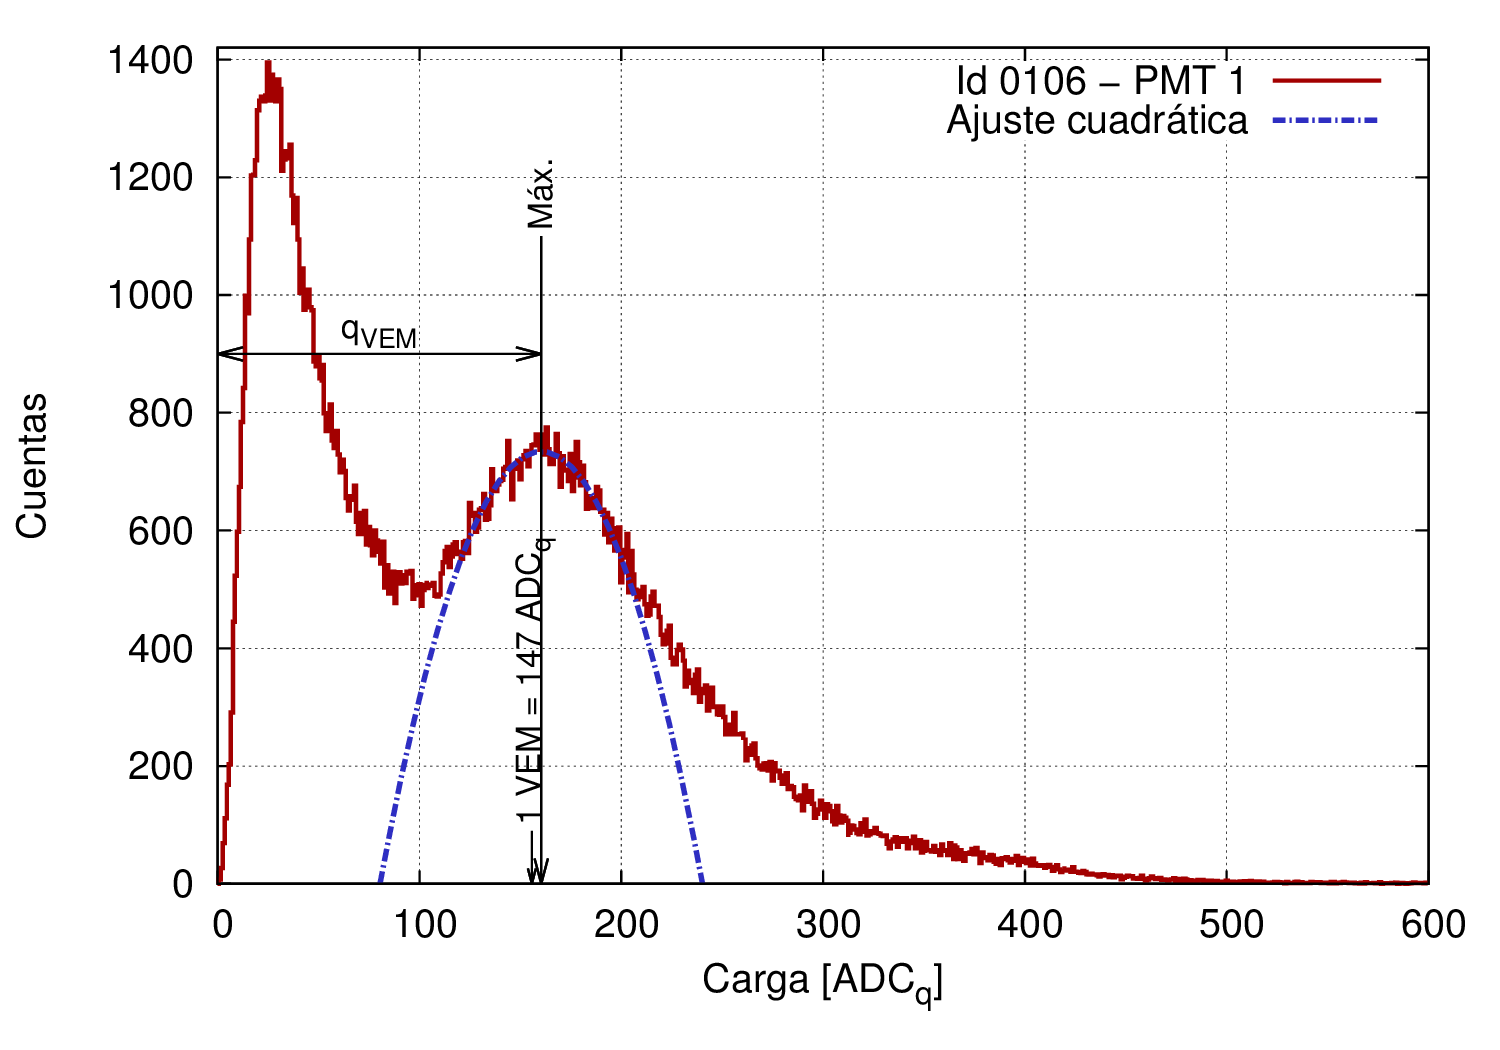
\includegraphics[width=0.6\textwidth]{Figs/histograma_carga.png}
  \caption{Carga depositada durante un tiempo y medida por un tubo fotomultiplicador del observatorio. El pico inicial refleja la distribución de señales principalmente generadas por la componente electromagnética, sumada al efecto del umbral de detección. El segundo pico, por su parte, se relaciona con el paso de muones que atraviesan verticalmente el detector. Fuente: (\cite{asorey_2012})}
  \label{cargahist}
\end{figure}
Algunos parámetros de importancia referentes a los detectores Cherenkov del Observatorio que serán necesarios para las secciones siguientes son:
\begin{itemize}
\item     \textbf{Bin de la señal:} Intervalo entre dos pulsos sucesivos. Considerando que el conversor tiene una tasa de muestreo de 40MHz, se establece que $1bin\equiv \frac{1}{40MHz} = 25ns$
    \item \textbf{Cuentas ADC de pico:} Es la magnitud correspondiente al valor de salida del conversor FADC de tal forma que $1ADC_{p}= 1.95mV$ 
    \item \textbf{Cuenas ADC de carga:} Unidad luego de integrar temporalmente la señal en $ADC_{p}$, restando la línea base.
    \item \textbf{$VEM$ (\textit{Vertical Equivalent Muon}):} Es la carga total depositada por un muón que atraviesa completamente a un detector de superficie de forma vertical, un $VCM$ (\textit{muón central y vertical}). $1VEM=\frac{q_{VEM}}{1.03}ADC_{q}=240MeV$.
    \item \textbf{$VEM_{p}$:} Es el equivalente a la altura máxima del pulso típico de la señal producido por un $MCV$: $1VEM_{P}=\frac{I_{VEM}}{1.03}ADC_{p}=240MeV$.
    \item \textbf{Relación carga sobre pico $AoP$: } Es la relación de las cargas integradas $(ADC_{q})$ y los voltajes $(ADC_{p})$ en la zona de pico de muones del histograma de tal forma que: $AoP=\frac{ADC_{q}}{ADC_{p}}$ que correspondería a un parámetro fundamental de calibración. Con este parámetro posible tener una idea de la respuesta impulsional del detector frente a los muones, relacionando con cargas integradas.
    \item \textbf{Sistema de umbral (trigger):} Es la estructura de 5 niveles que se establecen sobre el nivel de detección para seleccionar las señales producidas por los CR de interés sobre el fondo, con el objetivo de descartar ruidos y eventos físicos no relevantes para el observatorio. A partir del sistema de Trigger se logra registrar de forma diaria un promedio de 3 eventos por detector (\cite{asorey_2012}).
\end{itemize}

\section{Medición del fondo de CR}

El fondo de CR secundarios en la superficie de la Tierra es el resultado de las interacciones de los CR galácticos (GCRs) y el viento solar con la atmósfera terrestre. Podría decirse que este fondo corresponde a un flujo constante de partículas que varía levemente debido a la actividad solar periódica y transitoria (\cite{masias_2017}). El Observatorio Pierre Auger, aunque está optimizado para la identificación de partículas de ultra alta energía, tiene dos modos de detección alternativos de baja energía que registran el flujo de partículas secundarias al nivel de los detectores de superficie: El modo scaler y el modo Histograma. En  este trabajo de investigación exploramos las características y propiedades del modo scaler aplicado al estudio del fondo de radiación natural y su variabilidad estrechamente relacionada con la actividad solar, aprovechando la capacidad de recolección de datos, la cantidad de detectores y la superficie cubierta por este arreglo.

\subsection{Modo scaler}

En 1997, se propuso la implementación en el observatorio de un modo de detección que estuviera destinado a caracterizar el fondo y  con este, identificar lluvias atmosféricas extendidas originadas por los fotones provenientes de GRBs (destellos de rayos gamma)(\cite{asorey_2012} , \cite{bertou_2011}). Los GRB consisten en una emisión súbita de rayos gamma en periodos cortos de tiempo ($\cdot 10^{-3}s - \cdot 10^{2}s$) que continúa en la emisión de fotones cada vez menos energéticos (rayos X hasta radio). El espectro en energía de los fotones gamma observados durante la ocurrencia de un GRB, muestran que podrían llegar hasta energías de varios GeV (\cite{Bernlöhr_1996}).
%El espectro de energía de los fotones gamma que han sido observados y reportados pueden llegar a energías en el rango de unidades de $GeV$ 

De esta forma se crea el modo scaler que consiste en determinar las tasas de conteo de pulsos individuales de cada detector de superficie en escalas de tiempo de un segundo \cite{asorey_2012}. Con este método, se puede determinar el flujo de fondo sobre el arreglo y a partir de éste, identificar excesos generados por fenómenos transitorios diversos como los GRB y también pueden dar una idea de la tasa de CR de baja energía influenciados por la modulación solar.

Como es de esperarse, no todas las señales registradas en el detector corresponden a datos válidos para la determinación de este flujo. En primer lugar, la diferencia entre la línea base y el voltaje del pico del pulso debe cumplir las siguientes condiciones:

\begin{itemize}
    \item Del 20 de Marzo hasta el 20 de Septiembre de 2005, este voltaje debe ser mayor a 3ADC
    \item Desde el 21 de Septiembre del 2005, la diferencia de voltajes debe comprender entre: $3ADC < (V_{p}-V_{b}) \leq 20ADC $
\end{itemize}

Esta diferencia de periodos se sustenta en la necesidad de implementar un umbral de detección superior que permita una mejor relación señal a ruido \cite{bertou_2007}, y así superar las limitaciones en los datos que se venían recolectando. Dichos cambios en los umbrales fueron implementados desde el 21 de Septiembre del 2005.

Los pulsos recopilados son guardados enviados una vez por segundo para su almacenamiento. Cada segundo de datos contiene: el tiempo en que se realizó el registro, número de estaciones activas, el número total de pulsos contados en todo el arreglo, y los conteos de pulsos para cada detector. Finalmente se obtiene un archivo de datos por día. Luego de esto, se deben eliminar los detectores que muestren inestabilidades respecto a la media, ruido producido por rayos, inestabilidades térmicas y relámpagos originados en tormentas eléctricas.  

\subsection{Modo histograma}

El modo Histograma permite estudiar la variación de la tasa de conteo en diferentes rangos de energía depositada, asociados con diversas energías primarias de GCR. En el sistema de detección del Observatorio, corresponde al registro de los pulsos del fondo de radiación en intervalos de tiempo de 61 segundos \cite{asorey_2012} . Estos registros permiten realizar la calibración del detector en un intervalo de tiempo determinado respecto a su respuesta impulsional y acompañan los eventos filtrados y almanecados por el sistema de trigger principal. 

Después del proceso de calibración, a partir del VEM se pueden construir histogramas de energía depositada de hasta aproximadamente 1 GeV. El modo Histograma permite estudiar la variación de la tasa de conteo en diferentes rangos de energía depositada, asociados con diversas energías primarias de CR galácticos (GCRs) (\cite{asorey_2012}, \cite{masias_2017}). Los dos rangos de energía de mayor interés son: el rango asociado a las energías depositadas en el modo scaler (energía entre 60 MeV y 120 MeV), y el relacionado con las energías depositadas por muones con incidencia vertical (energía entre 200 MeV y 280 MeV), también denominado \textit{banda muónica}. 

Los modos scaler e histograma están fuertemente relacionados puesto que la integral del histograma de carga, por construcción, representa el número de señales registradas en ese minuto. Ajustando adecuadamente los límites de esta integración, teóricamente debería ser posible recuperar las tasas de los scalers de ese detector (\cite{Martin_Schimassek2022}).